\subsection{Übertragen der Config Files mittels USB}
Um dem Programm die neuesten Konfigurationsdateien zu übergeben, steckt man beim Bootvorgang des Raspberry Pi einen Datenträger (\zB USB-Stick) an. Auf dem Datenträger muss im Root-Verzeichnis (\textasciitilde) ein Verzeichnis namens \enquote{RLT\_Config} sein. Wenn dieses Verzeichnis und alle nötigen Konfigurationsdateien darin vorhanden sind, werden diese in das Documents Verzeichnis des Raspberry Pi kopiert. \newline Folgendes Aktivitätsdiagramm verdeutlicht diesen Vorgang. (Siehe Abb.~\ref{fig:config_ubertragen_activity}):
\begin{figure}[H]
	\centering
	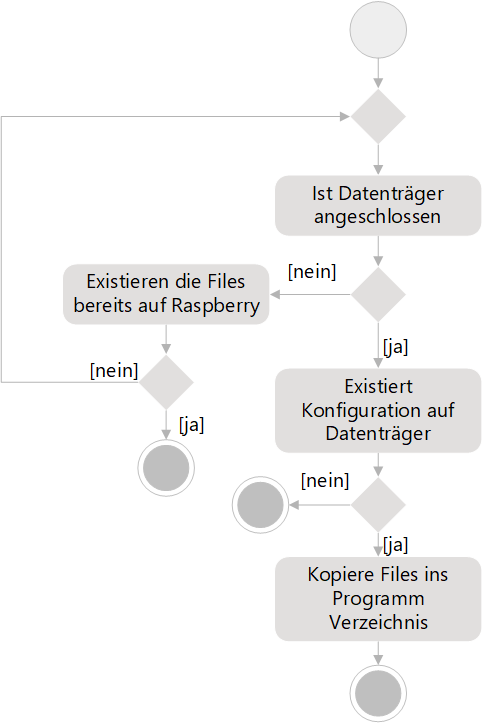
\includegraphics[width=0.4\linewidth]{Bilder/config_ubertragen_activity_diagram}
	\caption{Übertragen der Konfigurationsdateien}
	\label{fig:config_ubertragen_activity}
\end{figure}

%\pythonfile[firstline=2, lastline=12]{Code/main.py}

Das passiert in der \enquote{usb\_routine} Funktion. Diese Funktion liefert einen Fehlercode zurück, der daraufhin in einer Verzweigung abgefragt wird. Wenn ein Fehler beim Übertragen auftritt, terminiert das Programm. Ansonsten fährt das Programm fort.

\begin{pythoncode}
if __name__ == "__main__":
	copy_error = usb_detection.usb_routine()
	if copy_error:
		exit
	all_pages = modbus.load_config()
	global app
	app = App(all_pages)
	setup_buttons()
	modbus.data_threading(app)
	app.mainloop()	
\end{pythoncode}

Es wird die \enquote{copy\_from\_usb} Funktion aufgerufen. Diese gibt einen Statuscode zurück. Die \enquote{start\_window} Funktion erstellt ein neues customtkinter Fenster, in dem dann der Parameter string angezeigt wird. Das Fenster bleibt für sieben Sekunden offen, bevor es wieder geschlossen wird und die Ausführung fortfährt.

\begin{pythoncode}
def usb_routine():
	copy_error = copy_from_usb()
	if copy_error == -1:
		return True
	elif copy_error == 0:
		start_window("Config Dateien wurden kopiert. Entferne nun den USB")   
	elif copy_error == 1: 
		start_window("Kein USB-Stick gefunden und Config bereits vorhanden")  
	return False
\end{pythoncode}

Es folgt die Beschreibung der \enquote{copy\_from\_usb} Funktion. Es wird geschaut ob auf einem der sd-Ports ein Datenträger angeschlossen ist. Wenn ja, wird der entsprechende Port gespeichert und die Abfrage beendet. Wenn kein Datenträger gefunden wird, kann man davon ausgehen, dass keine Änderung an der Konfiguration vorgenommen werden soll. Es wird nun überprüft, ob im Programmverzeichnis alle benötigten Konfigurationsdateien vorhanden sind. Das passiert im \enquote{check\_if\_files\_exists}. Wenn ja, ist der Kopiervorgang abgeschlossen, wenn nein, wird der Vorgang wiederholt, bis ein Datenträger gefunden wird. Die Ausführung wird für fünf Sekunden gestoppt, damit der Benutzer oder die Benutzerin genügend Zeit hat einen Datenträger einzufügen.

\begin{pythoncode}
	port = ""
	while True:
		if (os.system("mount | grep sda1") != 256):
			port = "sda1"
			break
		elif (os.system("mount | grep sdb1") != 256):
			port = "sdb1"
			break
		elif (os.system("mount | grep sdc1") != 256):
			port = "sdc1"
			break
		elif (os.system("mount | grep sdd1") != 256):
			port = "sdd1"
			break
		
		if (check_if_files_exists(config_path, device_config_path, False)):
			return 1
			
		time.sleep(5)
\end{pythoncode}

Wenn ein Datenträger gefunden wurde, wird dieser Port gemountet. Dieses mal wird überprüft, ob die Konfigurationsdateien auf dem Datenträger existieren. Wenn nicht, wird der Datenträger ausgeworfen und ein Fehlercode zurückgegeben. Ansonsten werden die Dateien kopiert und der Datenträger ausgeworfen. Die beiden Funktionen \enquote{check\_if\_files\_exists} und \enquote{start\_window} sind im Codeanhang zu finden. Beim Auswerfen wird manchmal eine Nachricht angezeigt, dass der Datenträger nicht ausgeworfen wurde. Dies kann ignoriert werden (Quelle angeben; falls das überhaupt stimmt).

\begin{pythoncode}
	os.system("sudo umount /dev/" + port)
	os.system("sudo mount /dev/" + port + " /home/pi/Documents/Config")
	
	error_free = check_if_files_exists(usb_config_path, usb_device_config_path, True)
	if error_free:
		os.system("cp -r ~/Documents/Config/RLT_Config ~/Documents/")
	else:
		os.system("sudo umount /dev/" + port)
		#os.system("sudo eject /dev/" + port) 
		#os.system("udisk --detach /dev/" + port)
		return -1
		
	os.system("sudo umount /dev/" + port)
	#os.system("sudo eject /dev/" + port) 
	#os.system("udisk --detach /dev/" + port)
	return 0
\end{pythoncode}